\documentclass{efd-lecture}

\begin{document}

\begin{frame}
  \titlepage{}
\end{frame}
\begin{frame}
  \frametitle{Outline}
  \tableofcontents{}
\end{frame}

\section{Introduction}

\section{JSON Schema}

\begin{frame}
  \frametitle{JSON Schema}
  \begin{itemize}
    \item JSON schema is JSON also
    \item The JSON document being validated or described we call the
      \textit{\color{YellowOrange} instance}, and the document containing the
      description is called the \textit{\color{GreenYellow} schema}.
  \end{itemize}
\end{frame}

\begin{frame}[fragile]
  \frametitle{Hello World}
  \begin{itemize}
    \item This accepts anything, as long as it’s valid JSON
      \mint[bgcolor=Black]{json}|{}|
    \item The most common thing to do in a JSON Schema is to restrict to a specific type. The \textit{\color{YellowOrange} type} keyword is used for that.
    \begin{minted}[bgcolor=Black]{json}
{ "type": "string" }
    \end{minted}
  \end{itemize}
\end{frame}

\begin{frame}[fragile]
  \frametitle{Declaring a JSON Schema}
  \begin{itemize}
    \item It's generally good practice to include it, though it is not required.
    \item The \textit{\color{YellowOrange} \$schema} keyword is used to declare
        that something is JSON Schema.
    \item Since JSON Schema is itself JSON, it's not always easy to tell when
        something is JSON Schema or just an arbitrary chunk of JSON.
  \end{itemize}
  \begin{minted}[bgcolor=Black]{json}
{ "$schema": "http://json-schema.org/draft-07/schema#" }
{ "$schema": "http://json-schema.org/draft/2019-09/schema#" }
  \end{minted}
\end{frame}

\begin{frame}[fragile]
  \frametitle{Declaring a unique identifier}
  \begin{itemize}
    \item It is also best practice to include an
      \textit{\color{YellowOrange} \$id} property as a unique identifier for
      each schema.
    \item For now, just set it to a URL at a domain you control, for example:
  \end{itemize}
  \begin{minted}[bgcolor=Black]{json}
{ "$id": "http://yourdomain.com/schemas/myschema.json" }
  \end{minted}
\end{frame}

\section{Swagger}

\section{AsyncAPI}

\begin{frame}
  \frametitle{Event-Driven Architectures}
  \begin{itemize}
    \item In most cases, Event-Driven Architectures (EDAs) are broker-centric.
    \item A message broker (or "broker") is a piece of infrastructure in charge of receiving messages and delivering them to those who have shown interest.
  \end{itemize}
  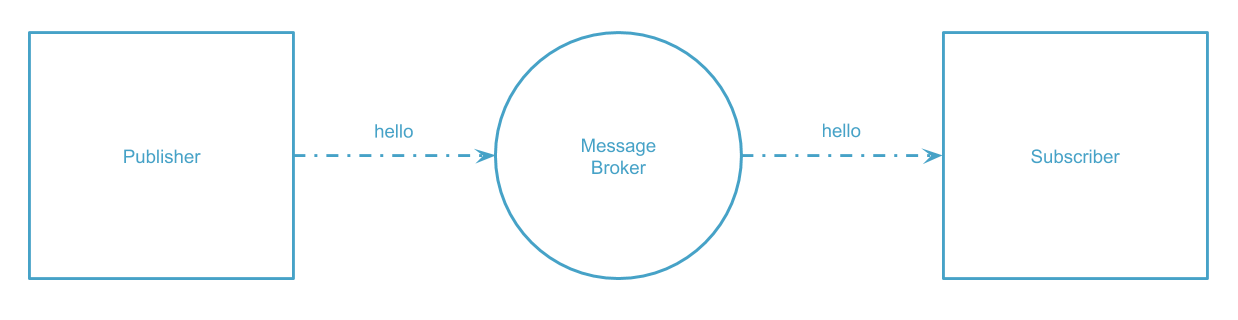
\includegraphics[width=\textwidth]{./img/simple-event-driven.png}
\end{frame}

\begin{frame}[fragile]
  \frametitle{Hello World}
  \begin{minted}[bgcolor=Black]{yaml}
asyncapi: 2.2.0
info:
  title: Hello world application
  version: '0.1.0'
channels:
  hello:
    publish:
      message:
        payload:
          type: string
          pattern: '^hello .+$'
  \end{minted}
\end{frame}

\begin{frame}[fragile]
  \frametitle{Hello World (Cont'd)}
  \begin{block}{}
    The first line of the specification starts with the document type \textit{\color{YellowOrange} asyncapi} and the version (2.2.0).
    This line doesn't have to be the first one,
    but it's a recommended practice.
  \end{block}
\end{frame}

\begin{frame}[fragile]
  \frametitle{Hello World (Cont'd)}
  \begin{block}{}
    The \textit{\color{YellowOrange} info} object contains the minimum required information about the application.
    It contains the \textit{\color{YellowGreen} title}, which is a memorable name for the API, and the version. While it's not mandatory,
    it's strongly recommended to change the \textit{\color{YellowGreen} version} whenever you make changes to the API\@.
  \end{block}
\end{frame}

\begin{frame}[fragile]
  \frametitle{Hello World (Cont'd)}
  \begin{block}{}
    The channels section of the specification houses all of the mediums where messages flow through. For example,
    some systems use topic, event name or routing key.
    Different kinds of information flow through each channel similar to the analogy of TV channels.
  \end{block}
\end{frame}

\begin{frame}
  \begin{block}{}
    This is the payload of the message that the Hello world application is subscribed to.
    You can publish the message to the hello channel and the Hello world application will receive it.
  \end{block}
\end{frame}

\begin{frame}
  \frametitle{Channels}
  \begin{description}
    \item[subscribe] A definition of the \textsc{\color{YellowOrange}Subscribe} operation, which defines the messages produced by the application and sent to the channel.
    \item[publish] A definition of the \textsc{\color{LimeGreen}Publish} operation, which defines the messages consumed by the application from the channel.
    \item[bindings] A map where the keys describe the name of the \textit{\text{Cyan}protocol} and the values describe protocol-specific definitions for the channel.
    \item[parameters] A map of the parameters included in the \textbf{\color{Purple} channel name}.
  \end{description}
\end{frame}

\begin{frame}[fragile]
  \frametitle{Channels (Cont'd)}
  \scriptsize
  \begin{minted}[bgcolor=Black]{yaml}
description: This channel is used to exchange messages about users signing up
subscribe:
  summary: A user signed up
  message:
    description: A longer description of the message
    payload:
      type: object
      properties:
        user:
          $ref: "#/components/schemas/user"
        signup:
          $ref: "#/components/schemas/signup"
bindings:
  amqp:
    is: routingKey
    exchange:
      name: myExchange
      type: topic
      durable: true
      autoDelete: false
      vhost: /
  \end{minted}
\end{frame}

\begin{frame}[fragile]
  \frametitle{Channels (Cont'd)}
  \scriptsize
  \begin{minted}[bgcolor=Black]{yaml}
user/{userId}/signup:
  parameters:
    userId:
      description: Id of the user
      schema:
        type: string
  subscribe:
    message:
      $ref: "#/components/messages/userSignedUp"
  \end{minted}
\end{frame}

\section{Go}

\begin{frame}
  \frametitle{How to Run?}
  \begin{itemize}
    \item List the service dependencies
    \item Have a docker-compose with these dependencies
  \end{itemize}
\end{frame}

\begin{frame}
  \frametitle{Comment}
  \begin{itemize}
    \item Have comments on exported \textit{\color{YellowOrange}Fields}, \textit{\color{LimeGreen}Methods},
      \textit{\color{Cyan}Functions} and \textit{\color{RubineRed}Structs}.
  \end{itemize}
\end{frame}

\begin{frame}
  \frametitle{Have everything on Git}
  \begin{itemize}
    \item \textbf{\color{RubineRed}Don't} relay on Environment variables because they don't have any documentation or history.
    \item \textbf{\color{RubineRed}Don't} store keys with Persons, they will forget it.
  \end{itemize}
\end{frame}

\section{Confluence}

\begin{frame}
  \frametitle{Do's and Don'ts}
  \begin{itemize}
    \item Use it for high-level architectures and meeting notes.
    \item \textbf{\color{RubineRed}Don't} store code-related things because they will be out of sync soon.
  \end{itemize}
\end{frame}

\end{document}
